%% Преамбула TeX-файла

% 1. Стиль и язык
\documentclass[utf8x]{G7-32} % Стиль (по умолчанию будет 14pt)
\usepackage[T2A]{fontenc}
\usepackage[russian]{babel}
% Остальные стандартные настройки убраны в preamble.inc.tex.
\sloppy

% Настройки стиля ГОСТ 7-32
% Для начала определяем, хотим мы или нет, чтобы рисунки и таблицы нумеровались в пределах раздела, или нам нужна сквозная нумерация.
\EqInChapter % формулы будут нумероваться в пределах раздела
\TableInChapter % таблицы будут нумероваться в пределах раздела
\PicInChapter % рисунки будут нумероваться в пределах раздела

% Добавляем гипертекстовое оглавление в PDF
\usepackage[
bookmarks=true, colorlinks=true, unicode=true,
urlcolor=black,linkcolor=black, anchorcolor=black,
citecolor=black, menucolor=black, filecolor=black,
]{hyperref}

% Изменение начертания шрифта --- после чего выглядит таймсоподобно.
% apt-get install scalable-cyrfonts-tex

\IfFileExists{cyrtimes.sty}
    {
        \usepackage{cyrtimespatched}
    }
    {
        % А если Times нету, то будет CM...
    }

\usepackage{graphicx}   % Пакет для включения рисунков

% С такими оно полями оно работает по-умолчанию:
% \RequirePackage[left=20mm,right=10mm,top=20mm,bottom=20mm,headsep=0pt]{geometry}
% Если вас тошнит от поля в 10мм --- увеличивайте до 20-ти, ну и про переплёт не забывайте:
\geometry{right=20mm}
\geometry{left=30mm}


% Пакет Tikz
\usepackage{tikz}
\usetikzlibrary{arrows,positioning,shadows}

% Произвольная нумерация списков.
\usepackage{enumerate}

% ячейки в несколько строчек
\usepackage{multirow}

% itemize внутри tabular
\usepackage{paralist,array}


% Полезные макросы листингов.
% Любимые команды
\newcommand{\Code}[1]{\textbf{#1}}

%% Перенос знаков в формулах (по Львовскому)
\newcommand*{\hm}[1]{#1\nobreak\discretionary{}
{\hbox{$\mathsurround=0pt #1$}}{}}


\begin{document}

\frontmatter % выключает нумерацию ВСЕГО; здесь начинаются ненумерованные главы: реферат, введение, глоссарий, сокращения и прочее.

% Команды \breakingbeforechapters и \nonbreakingbeforechapters
% управляют разрывом страницы перед главами.
% По-умолчанию страница разрывается.

% \nobreakingbeforechapters
% \breakingbeforechapters


\tableofcontents

\Abbreviations %% Список обозначений и сокращений в тексте
\begin{description}
\item[ООН] Организация Объединённых Наций.
\item[МВФ] Международный Валютный Фонд.
\item[ВВП] Валовой внутренний продукт.
\item[ИТ] Информационные технологии.
\item[RSD] Сербский динар.
\item[USD] доллар США.
\item[НАТО] Организация Североатлантического договора, Североатлантический Альянс (англ. North Atlantic Treaty Organization).
\item[ПИИ] Прямые иностранные инвестиции.
\item[США] Соединенные Штаты Америки.
\end{description}

%%% Local Variables:
%%% mode: latex
%%% TeX-master: "rpz"
%%% End:

\Introduction

Республика Сербия --- индустриально-аграрная страна, расположенная на юго-востоке Европы (Западные Балканы).
Республика является связывающим звеном между Центральной Европой и Ближним Востоком.
Через страну проходят торговые и транспортные пути.
Республика Сербия имеет запасы полезных ископаемых --- руды цветных металлов, каменный уголь и т.~д.
Через страну протекают крупные реки (Дунай, Сава, Дрина и т.~д.).

На рубеже 1980 -- 1990 годов страна (на тот момент Югославия) была экономически развитой.
Однако политические события 90-х (уничтожение промышленности в ходе многочисленных воздушных атак НАТО, война, санкции ООН, утрата всех связей внутри бывшей Югославии и т.~д.) оказали негативное влияние на экономическое и политическое положение страны.

За последние годы в Сербии начался стремительный экономический рост, возобновились иностранная финансовая помощь и инвестиции.
За 10-летний период по данным МВФ сербская экономика выросла почти на 20 процентов.

Сельское хозяйство, промышленность и сектор услуг являются основными источниками доходов Сербии.
Они внесли большой вклад в динамику роста ВВП.
Основная отрасль сельского хозяйства --- растениеводство.
В обрабатывающей промышленности ведущее место занимают машиностроение и металлообработка.
Также уверенными темпами развиваются ИТ и туризм.
Например, экспорт ИТ сектора в 2019 году был выше, чем экспорт доминирующего сельского хозяйства.
Примечательно, что в 2019 году Балканская республика наряду с Ирландией показала самый высокий экономический рост среди всех остальных государств Европы.
В 2020 году Сербия также может показать опережающию темпы роста экономики в Европе.

\textbf{Актуальность выбранной темы выпускной квалификационной работы } обусловлена тем, что экономика Сербии в настоящий момент находится на этапе активного развития.
Математические модели способны описать текущую экономическую ситуацию в стране и спрогнозировать как и положительные, так и отрицательные сюжеты развития государства.

Экономика государства очень сильно зависит от политической ситуации, она настолько динамична, что построив математическую модель вчера, сегодня она уже может оказаться не актуальной. В связи с вспышкой пандемии COVID-19\footnote{COVID-19 (аббревиатура от англ. COronaVIrus Disease 2019), коронавирусная инфекция 2019-nCoV --- потенциально тяжёлая острая респираторная инфекция, вызываемая коронавирусом \cite{wiki:Coronavirus_disease_2019}.}, многие страны уже оказались в неприятной экономической ситуации.
Это еще одна причина выбора темы.
Кроме того, построение математических моделей экономики государства на примере Сербии поможет разобраться как в особенностях государства, так и в математических инструментах.

\textbf{Объект исследования} --- математические модели экономического роста.

\textbf{Предмет исследования} --- математическая модель экономики, построенная на примере Республики Сербия.

\textbf{Цель данной работы} --- смоделировать динамику экономики Республики Сербия в зависимости от поведения внутренних и внешних переменных и сделать выводы.

Для реализации поставленной цели необходимо решить следующие задачи:
\begin{enumerate}
	\item Изучить теорию построения математических моделей экономики.
	\item Построить модель на примере макроэкономических данных Республики Сербия.
	\item Сделать выводы.
\end{enumerate}

Выпускная квалификационная работа состоит из содержания, перечня сокращений, введения, пяти глав, заключения, списка используемых источников и приложения.

В первой главе определяются основные термины, описываются этапы построения математических моделей, приводятся различные типы математических моделей.

Во второй главе описывается теоретическая состовляющая математической модели экономического роста Солоу.

В третьей главе рассчитываются основные макроэкономические переменные экономики Республики Сербия.

В четвертой главе проводится анализ, вычисления и построение математической модели экономики Республики Сербия, разбираются полученные результаты.

В пятой главе исследуются главные сферы экономической деятельности Сербии, оцениваются прогнозы авторитетных рейтинговых агенств (МВФ, Всемирный банк и т.~д.).


\mainmatter % это включает нумерацию глав и секций в документе ниже
\chapter{Понятие математической модели}
\label{cha:definition}

\section{Основные понятия}

Объект --- система состоящая из множества элементов.
Это может быть ракета, рынок ценных бумаг или популяции животных.
В нашем случае это государство.

Модель несет в себе отражение связей между элементами.
Математическая модель --- это математическое представление реальности.
Экономической моделью можно считать набор уравнений, основанных на определенных предположениях и приближено описывающих экономику в целом или отдельно ее отрасль.

Моделирование --- процесс расчета поведения системы на основе граничных условий и заданных связей между элементами системы.

Алгоритм --- логика расчета поведения системы.
Логика может быть основана на разных математических подходах.

\section{Этапы построения математической модели}

Построение математических моделей в экономике является методом для решения задач оптимального упраления.
Экономико-математическая модель отображает некоторые процессы, которые смоделированы с помощью математических теорем и уравнений.

Построение математических моделей состоит из нескольких этапов:
\begin{itemize}
	\item \textbf{Идентификация.}
	Определение основных параметров объекта.
	\item \textbf{Оценка параметров модели.}
	Выбор переменных модели на основе выбранных параметров.
	\item \textbf{Спецификация модели.}
	Определение связей между параметрами.
	Построение уравнений.
	\item \textbf{Моделирование.}
	Проведение моделирования на основе заданных начальных условий.
	\item \textbf{Анализ полученных результатов.}
\end{itemize}

\section{Классификация математических моделей}

Формальная классификация моделей основывается на классификации используемых математических средств.
Например:
\begin{itemize}
	\item \textbf{Линейные и нелинейные модели.}
	Модели, в которых связь между зависимой и независимой переменными могут быть линейными или нелинейными (например, линейная регрессия).
	\item \textbf{Дискретные и непрерывные модели.}
	В дискретных моделях изменение параметров связано только с отдельными моментами времени.
	В непрерывных моделях параметры изменяются во времени плавно.
	\item \textbf{Стохастические модели.}
	Стохастические модели предназначены для прогнозирования экономических явлений в условиях неопределенности исходных данных и реализуются методами математической статистики.
	\item \textbf{Оптимизационные модели.}
	Оптимизационная модель позволяет из нескольких альтернативных вариантов выбрать наилучший вариант по любому признаку.
\end{itemize}

Естественно, что существуют и другие модели, в том числе и смешанные.

\chapter{Анализ развития экономики в Республике Сербия}
\label{cha:analys}

В настоящее время наблюдается явная нехватка эконометрических работ, связанных с построением математических моделей экономики различных государств.
Однако многие рейтинговые агенства регулярно прогнозируют различные варианты развития государства, пишут отчеты, строят стратегии экономичекого роста и т.~д.

\section{Текущая экономическая ситуация в Республике Сербия}

Рост в Республике Сербия в 2019 году несколько снизился по сравнению с 2018 годом, но оставался устойчивым на уровне 4,2 процента, что обусловлено увеличением государственных инвестиций наряду с высокими показателями ПИИ.

Потребление оставалось на высоком уровне.
Вклад чистого экспорта в рост был отрицательным, поскольку экспорт рос не так быстро, как в прошлых годах.
Если посмотреть на отраслевой состав, то в 2019 году промышленность увеличилась всего на 0,3 процента, а объем производства в сельском хозяйстве в целом остался таким же, как в 2018 году.
Однако, наряду со строительным сектором, услуги внесли значительный вклад в рост ВВП.

Уровень активности и уровень занятости среди населения в возрасте 15 лет и старше в четвертом квартале 2019 года продолжали расти.
Уровень безработицы снизился до 9,7 процента в последнем квартале 2019 года.

Благодаря этим тенденциям уровень бедности\footnote{Доход ниже 5,5 долларов США в день --- стандартизированная черта бедности в странах со средним уровнем дохода.} снизился с 25,8 процента в 2015 году до примерно 18,9 процента в 2019 году.

К концу 2019 года государственный долг Сербии сократился до 52,9 процента ВВП.
Инфляция была низкой и стабильной.
%При низком инфляционном давлении \nom{НБС}{Народный банк Сербии} понизил свою учетную ставку до 1,75 процента в марте 2020 года.

Приток ПИИ оставался высоким в 2019 году.
Общий объем кредитов вырос на 8,5 процента, в то время как просроченные кредиты сократились до 4,1 процента в декабре 2019 года.

\section{Стратегия развития Всемирного банка}

Согласно отчетам Всемирного банка экономика Сербии может расти быстрее, чем в настоящее время (3 -- 4 процента в год).
В отчете \cite{worldbank_cem} и связанных с ним документах \cite{worldbank_investment,worldbank_financing, worldbank_productivity, worldbank_encouraging, worldbank_labormarket, worldbank_barriers, worldbank_aid, worldbank_workforce} изложена стратегия, которая может помочь экономике страны расти быстрее.
Всемирный банк считает, что текущие темпы роста недостаточно быстро приближают страну к среднему уровню жизни в Европейском Союзе.
Опираясь на новую стратегию Сербия может расти в среднем на 7 процентов в год, удваивоив свои доходы за 10 лет.

В стратегии намечены семь ключевых шагов, которые могли бы привести экономику страны к указанным темпам роста.
В частности:
\begin{itemize}
	\item \textbf{Увеличение инвестиций.}
	Увеличение государственных и частных инвестиций поддержит стабильность высоких темпов роста.
	\item \textbf{Финансирование для растущих фирм.}
	Увеличение кредита частному сектору до уровня, близкого к европейским стандартам, расширит финансирование для малых и средних предприятий.
	\item \textbf{Квалифицированные рабочие.}
	Поскольку более двух третьих фирм не могут найти работников для расширения, повышение качества образования может увеличить темпы роста ВВП.
	\item \textbf{Повышение производительности.}
	Повышение производительности труда позволит увеличить производство с добавленной стоимостью, увеличить количество рабочих мест и повысить заработную плату.
	\item \textbf{Содействие экспорту.}
	Сербские экспортеры в среднем в два раза продуктивнее других фирм.
	Улучшение инфраструктуры и устранение таможенных ограничений будут способствовать увеличению экспорта.
	\item \textbf{Улучшение правоприменения.}
	Усовершенствованная нормативно-правовая база, предсказуемость и прозрачность административных процедур могли бы сократить расходы для бизнеса.
	\item \textbf{Развязывание конкуренции.}
	Сокращение государственного присутствия в экономике уменьшит барьеры для конкуренции.
\end{itemize}

\section{Экономический прогноз}

Вспышка пандемии COVID-19\footnote{COVID-19 (аббревиатура от англ. COronaVIrus Disease 2019), ранее коронавирусная инфекция 2019-nCoV — потенциально тяжёлая острая респираторная инфекция, вызываемая коронавирусом \cite{wiki_covid}.} и связанные с ее распространением ограничительные меры наносят тяжелый урон как мировой экономике, так и экономике Республики Сербия.
Таким образом, экономический рост в стране может оказаться более низким, чем ожидалось ранее.
Снижение туристической и транспортной активности, сокращение денежных переводов, замедление экспорта и уменьшение ПИИ и инвестиций в целом могут привести экономику страны к рецессии в 2020 году.
Сербские власти принимают всесторонние меры для смягчения негативных последствий пандемии.

В среднесрочной перспективе (2021 -- 2023) рост может вернуться к прежней траектории.
Этот прогноз в решающей степени зависит от международных событий, темпов структурных реформ и политических событий.

Ожидается, что текущие события приведут к небольшому росту уровня бедности в 2020 году.
Помимо непосредственного воздействия на здоровье граждан, ожидаемое снижение инвестиций, сокращение спроса на сербский экспорт и ограничения мобильности нарушат ситуацию с рабочими местами и доходами.
Кризис, в первую очередь, затронет наиболее мелкие, уязвимые домохозяйства.
Глубина кризиса, прежде всего, будет зависеть от длительности пандемии COVID-19.
Текущий прогноз предполагает, что меры по сдерживанию могут быть постепенно отменены к концу второго квартала 2020 года.

Республика Сербия может сохранить свою с трудом завоеванную макроэкономическую стабильность и вывести свои экономические преобразования на новый уровень.
Таким образом, данная работа представляет интерес как для экономики Сербии, так и для академических кругов.

\chapter{Идентификация параметров модели}
\label{cha:ident_params}

Для построения математической модели используются макроэкономические показатели статистического агенства ООН \cite{unstat}.

Расчеты могут быть выполнены:
\begin{itemize}
	\item В долларах США.
	\item В национальной валюте.
\end{itemize}

Также существует два вида цен:
\begin{itemize}
	\item \textbf{Текущие.}
	Цены на какую-либо конкретную дату, например на 1 апреля, либо средние за год цены.
	\item \textbf{Постоянные.}
	Цены определенного периода, принимаемые за основу расчета макроэкономических показателей.
	Эти цены не учитывают уровень инфляции.
	На момент написания работы этот период --- 2015 год.
\end{itemize}
Если периоды текущих и постоянных цен совпадают, то и цены тоже соответственно совпадают.

Введем специальные обозначения, которые представлены в таблице \ref{tab:desig_of_params}.

\begin{table}[ht]
	\caption{Специальные обозначения для параметров}
	\begin{tabular}{|r|l|}
	\hline
	\multicolumn{1}{|r|}{Параметр} & \multicolumn{1}{l|}{Описание} \\ \hline
	$t$                          &Значение, получаемое при вычитании 2010 из текущего года\\
	$Y$                          & ВВП                                                   \\
	$I$                          & импорт                                                \\
	$J$                          & размер инвестиций                                     \\
	$C$                          & общие расходы на потребление                          \\
	$E$                          & экспорт                                               \\ \hline
	\end{tabular}
	\label{tab:desig_of_params}
\end{table}

Все переменные с нижним индексом $_{stat}$ обозначают статистические данные.
В противном случае, это параметры модели.
Переменные с нижним индексом $_{const}$ обозначают постоянные цены.
В противном случае текущие.

Таблицы найденных статистических данных для Республики Сербия  представлены в приложении \ref{cha:first_app}.
Все найденные показатели представлены в текущих и постоянных ценах.
Все данные представлены с 1993 года, так как это был переломный момент в истории страны.

Первым делом посчитаем индексы цен, определим поведение цен в среднем.
Индекс цен представляет собой соотношение макроэкономических показателей данного периода в текущих и постоянных ценах.
Для этого воспользуемся формулой:
\begin{equation}
	P(X(t)) = \cfrac{X(t)}{X_{const}(t)}
\label{F:F1}
\end{equation}
где $X(t)$ это макроэкономический показатель.

На Рис. \ref{fig:index_rsd} видна динамика поведения цен.
\begin{figure}
	\centering
	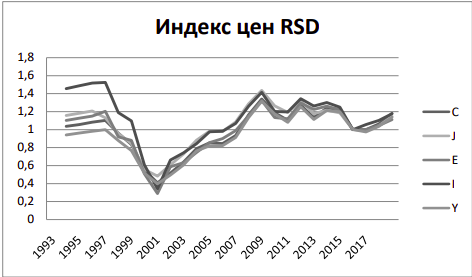
\includegraphics[width=\textwidth]{figures/index_rsd.png}
	\caption{Индекс цен RSD 1993 -- 2018}
	\label{fig:index_rsd}
\end{figure}

В дальнейшем все расчеты будут проведены в постоянных ценах национальной валюты 2015 года.

\backmatter %% Здесь заканчивается нумерованная часть документа и начинаются ссылки и

 %             %% заключение

\nocite{*}
\pagebreak
\printbibliography
\addcontentsline{toc}{section}{\refname}


\appendix   % Тут идут приложения

\chapter{Таблицы макроэкономических данных}
\label{cha:first_app}

В данном приложении приведены таблицы статистических макроэкономических показателей для Республики Сербия.

\begin{center}
\begin{longtable}{|r|c|c|c|c|l|}
	\caption{Макроэкономические показатели в текущих ценах RSD (млрд.).}
	\label{tab::gdp_cur_rsd}\\
	\hline
	Год & C   & J    & E       & I        & Y           \\ \hline
	\endfirsthead
	\subcaption{Продолжение таблицы~\ref{tab::gdp_cur_rsd}}
	\\ \hline \endhead
    \hline \subcaption{Продолжение на след. стр.}
    \endfoot
    \hline \endlastfoot
	\multicolumn{6}{|c|}{В текущих ценах --- Миллиарды сербских динаров}                             \\ \hline
	1993 & 28,56   & 3,57    & 3,68    & 6,75    & 30,60   \\
	1994 & 30,42   & 3,93    & 4,18    & 7,77    & 32,33   \\
	1995 & 54,91   & 6,74    & 4,81    & 8,96    & 59,30   \\
	1996 & 105,02  & 12,93   & 16,89   & 30,45   & 112,50  \\
	1997 & 137,59  & 19,36   & 22,36   & 42,67   & 142,77  \\
	1998 & 176,66  & 25,56   & 38,81   & 55,70   & 183,41  \\
	1999 & 208,37  & 28,66   & 25,19   & 39,47   & 214,68  \\
	2000 & 387,99  & 58,09   & 40,71   & 59,15   & 413,12  \\
	2001 & 788,84  & 105,80  & 184,23  & 309,82  & 820,84  \\
	2002 & 1005,78 & 168,01  & 214,28  & 401,93  & 1037,90 \\
	2003 & 1165,20 & 223,16  & 267,98  & 482,58  & 1220,16 \\
	2004 & 1401,40 & 298,45  & 351,53  & 734,92  & 1451,45 \\
	2005 & 1667,79 & 351,93  & 475,34  & 825,58  & 1751,37 \\
	2006 & 1958,49 & 457,76  & 622,03  & 1039,92 & 2055,20 \\
	2007 & 2241,71 & 595,03  & 667,99  & 1240,26 & 2355,07 \\
	2008 & 2598,91 & 684,66  & 799,24  & 1486,07 & 2744,91 \\
	2009 & 2778,75 & 566,16  & 773,20  & 1231,07 & 2880,06 \\
	2010 & 2960,46 & 570,06  & 1010,11 & 1469,85 & 3067,21 \\
	2011 & 3247,22 & 626,67  & 1157,76 & 1682,43 & 3407,56 \\
	2012 & 3428,60 & 758,70  & 1323,60 & 1921,03 & 3584,24 \\
	2013 & 3607,34 & 668,36  & 1597,09 & 2012,21 & 3876,40 \\
	2014 & 3648,67 & 652,01  & 1695,33 & 2119,29 & 3908,47 \\
	2015 & 3675,54 & 715,47  & 1887,24 & 2281,58 & 4043,47 \\
	2016 & 3929,03 & 766,31  & 2198,03 & 2415,48 & 4521,26 \\
	2017 & 4136,27 & 843,70  & 2402,90 & 2716,27 & 4754,37 \\
	2018 & 4351,18 & 1016,51 & 2573,60 & 3005,31 & 5068,59 \\ \hline
	\end{longtable}
\end{center}

\begin{center}
	\begin{longtable}{|r|c|c|c|c|l|}
		\caption{Макроэкономические показатели в постоянных ценах 2015 года RSD (млрд.).}
		\label{tab::gdp_const_rsd}\\
		\hline
		Год & C   & J    & E       & I        & Y           \\ \hline
		\endfirsthead
		\subcaption{Продолжение таблицы~\ref{tab::gdp_const_rsd}}
		\\ \hline \endhead
		\hline \subcaption{Продолжение на след. стр.}
		\endfoot
		\hline \endlastfoot
	\multicolumn{6}{|c|}{В постоянных ценах 2015 года --- Миллиарды сербских динаров}                             \\ \hline
	1993 & 1892,79   & 212,00  & 228,87   & 318,26   & 2231,47   \\
	1994 & 1960,79   & 226,33  & 252,62   & 355,45   & 2289,37   \\
	1995 & 2031,07   & 223,96  & 167,44   & 236,29   & 2419,57   \\
	1996 & 2097,59   & 251,88  & 309,11   & 439,65   & 2478,27  \\
	1997 & 2340,53   & 330,71  & 397,48   & 586,20   & 2656,33  \\
	1998 & 2404,54   & 343,93  & 501,14   & 576,47   & 2720,90  \\
	1999 & 2166,71   & 296,06  & 283,97   & 372,56   & 2390,40  \\
	2000 & 2351,13   & 297,88  & 348,16   & 427,30   & 2575,87  \\
	2001 & 2485,58   & 282,70  & 509,58   & 761,36   & 2704,48  \\
	2002 & 2660,40   & 389,77  & 572,99   & 916,52   & 2896,93 \\
	2003 & 2793,46   & 478,08  & 678,92   & 1081,69  & 3024,83 \\
	2004 & 3059,59   & 566,33  & 766,68   & 1404,04  & 3298,48 \\
	2005 & 3217,99   & 585,90  & 862,51   & 1373,28  & 3481,23 \\
	2006 & 3398,99   & 684,13  & 1020,72  & 1578,33  & 3651,97 \\
	2007 & 3585,92   & 860,96  & 1077,67  & 1831,95  & 3867,02 \\
	2008 & 3788,02   & 931,73  & 1178,84  & 2052,17  & 4074,55 \\
	2009 & 3769,47   & 721,67  & 1097,69  & 1649,35  & 3947,59 \\
	2010 & 3753,45   & 670,34  & 1262,47  & 1721,23  & 3970,66 \\
	2011 & 3788,63   & 705,27  & 1325,63  & 1856,82  & 4026,31 \\
	2012 & 3741,50   & 798,67  & 1336,24  & 1881,94  & 3985,43 \\
	2013 & 3716,74   & 702,74  & 1620,51  & 1976,92  & 4087,92 \\
	2014 & 3672,62   & 677,50  & 1712,50  & 2087,11  & 4013,05 \\
	2015 & 3675,54   & 715,47  & 1887,24  & 2281,58  & 4043,47 \\
	2016 & 3848,71   & 761,74  & 2146,99  & 2237,82  & 4541,58 \\
	2017 & 3932,67   & 817,67  & 2322,76  & 2486,88  & 4634,65 \\
	2018 & 4004,21   & 963,48  & 2515,65  & 2775,49  & 4838,21 \\ \hline
\end{longtable}
\end{center}

\begin{center}
	\begin{longtable}{|r|c|l|}
		\caption{Население Республики Сербия (млн.).}
		\label{tab::population}\\
		\hline
		Год & P   & L \\ \hline
		\endfirsthead
		\subcaption{Продолжение таблицы~\ref{tab::population}}
		\\ \hline \endhead
		\hline \subcaption{Продолжение на след. стр.}
		\endfoot
		\hline \endlastfoot
	\multicolumn{3}{|c|}{Миллионы человек}                             \\ \hline
	1993 & 9,80   & 3,41     \\
	1994 & 9,86   & 3,43     \\
	1995 & 9,88   & 3,38     \\
	1996 & 9,86   & 3,39    \\
	1997 & 9,78   & 3,38    \\
	1998 & 9,69   & 3,37    \\
	1999 & 7,55   & 3,38    \\
	2000 & 7,52   & 3,36    \\
	2001 & 7,50   & 3,35    \\
	2002 & 7,50   & 3,34   \\
	2003 & 7,48   & 3,33   \\
	2004 & 7,46   & 3,31   \\
	2005 & 7,44   & 3,30   \\
	2006 & 7,41   & 3,29   \\
	2007 & 7,38   & 3,29  \\
	2008 & 7,35   & 3,24   \\
	2009 & 7,32   & 3,14   \\
	2010 & 7,29   & 3,07   \\
	2011 & 7,24   & 3,05   \\
	2012 & 7,20   & 3,07   \\
	2013 & 7,17   & 3,12   \\
	2014 & 7,13   & 3,13   \\
	2015 & 7,10   & 3,09   \\
	2016 & 7,06   & 3,19   \\
	2017 & 7,04   & 3,22  \\
	2018 & 7,02   & 3,19   \\ \hline
\end{longtable}
\end{center}


\end{document}

%%% Local Variables:
%%% mode: latex
%%% TeX-master: t
%%% End:
